\documentclass[]{beamer}
\usepackage[T1]{fontenc}
\usepackage[utf8]{inputenc}
\usepackage{lmodern}
\usepackage[italian]{babel}
\usepackage{mathrsfs}
\usepackage{cancel}

\title{La fisica quantistica}
\author{\texorpdfstring{Mattia Cozzi\newline\href{mailto:cozzimattia@gmail.com}{\texttt{cozzimattia@gmail.com}}}{Mattia Cozzi}}
\date{a.s.~2023/2024}

%\documentclass[handout]{beamer}     %usare questa classe per generare l'handout
%\usepackage{pgfpages}   %per mostrare più quadri nella stessa pagina
%\pgfpagesuselayout{4 on 1}[a4paper,border shrink=5mm,landscape]
\usetheme{Singapore}
%\useoutertheme[left]{sidebar} %elementi intorno alle diapositive
\setbeamercovered{dynamic} %modifica l'aspetto del testo grigetto delle diapositive future. Argomenti: invisible/transparent/dynamic
\usecolortheme{orchid}
%COLORE PRINCIPALE
% \definecolor{marroncino}{RGB}{156, 26, 0} % UBC Blue (primary)
% \setbeamercolor{structure}{fg=marroncino} % itemize, enumerate, etc

\theoremstyle{plain}
\newtheorem{teorema}{Teorema}

\usepackage{tikz}
\usepackage{circuitikz}

\usepackage{pgf,pgfplots,graphicx}
\usetikzlibrary{angles,quotes,arrows,shapes,decorations.markings}
\pgfplotsset{compat=1.15}
\usepgfplotslibrary{units,fillbetween} % to add units easily to axis

\newcommand{\fem}{f_{em}}

\def\angolo[#1](#2)(#3:#4:#5)% Syntax: [draw options] (center) (initial angle:final angle:radius)
    { \draw[#1] ($(#2)+({#5*cos(#3)},{#5*sin(#3)})$) arc (#3:#4:#5); }


\newcommand<>{\xxcancel}[1]{\alt#2{\xcancel{#1}\vphantom{#1}}{#1}}

\begin{document}

\begin{frame}
  \titlepage
\end{frame}





\begin{frame}
\frametitle{Contenuti}
\tableofcontents
\end{frame}


\section{Dualismo (1)}


\begin{frame}
\frametitle{XVII secolo}
\begin{columns}
\begin{column}{0.2\textwidth}
\visible<1->{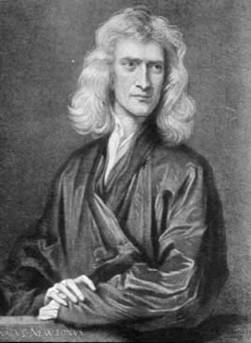
\includegraphics[width=\columnwidth]{img/newton.jpg}}
~
\visible<2->{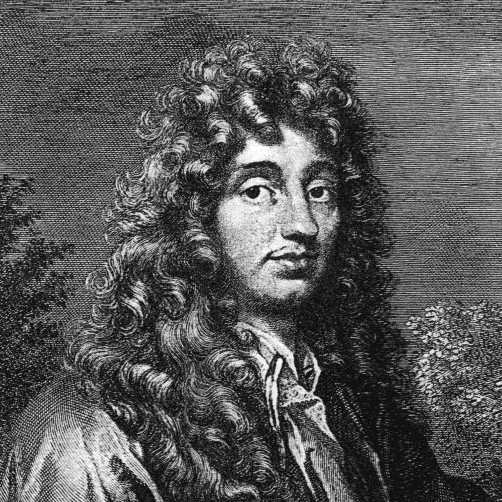
\includegraphics[width=\columnwidth]{img/huygens.jpg}}
\end{column}
\begin{column}{0.7\textwidth}
Nel XVII secolo furono proposte due teorie concorrenti in merito alla natura della luce:
\begin{itemize}
\item<1-> il \alert<1>{modello corpuscolare} di Newton (ispirato da Pierre Gassendi), per cui la luce è un flusso di particelle microscopiche emesse dalle sorgenti luminose;\pause
\item<2-> il \alert<2>{modello ondulatorio} di Huygens (ispirato da Robert Hooke), per cui la luce è un'onda (similmente al suono).
\end{itemize}

\end{column}
\end{columns}
\end{frame}


\begin{frame}
\frametitle{XIX secolo}
\begin{columns}
\begin{column}{0.2\textwidth}
\visible<1->{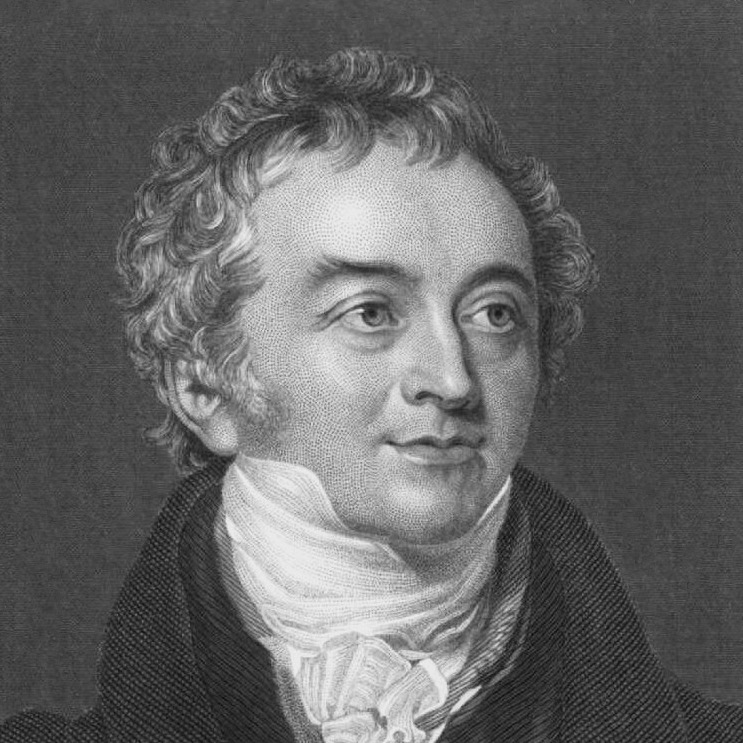
\includegraphics[width=\columnwidth]{img/young.jpg}}
~
\visible<3->{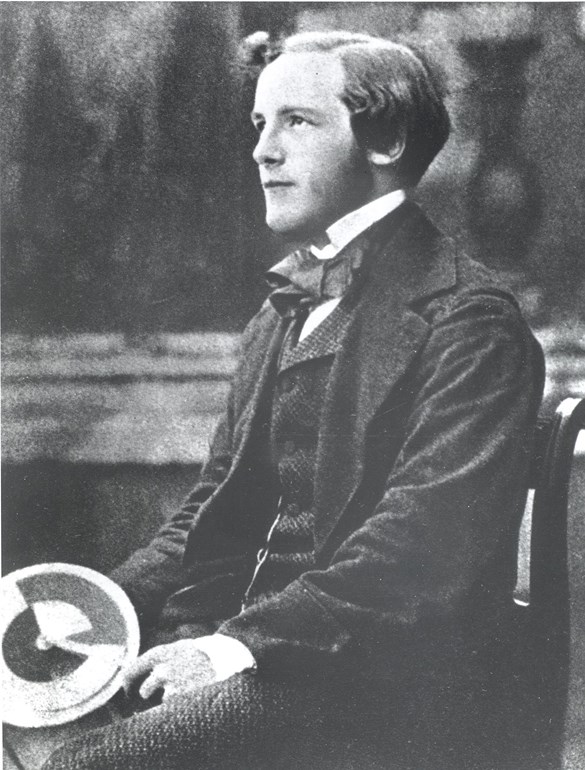
\includegraphics[width=\columnwidth]{img/maxwell.jpg}}
\end{column}
\begin{column}{0.7\textwidth}
Nel XVIII secolo prevale la teoria corpuscolare, ma:
\begin{itemize}
  \item<1-> Thomas Young (1801) dimostra che la luce presenta il \alert<1>{fenomeno dell'interferenza, tipico unicamente delle onde};
  \item<2-> Léon Foucault e Hippolyte Fizeau (1850) dimostrano che la luce nell'acqua è più lenta che nell'aria, \alert<2>{in accordo con la teoria ondulatoria};
  \item<3-> James Clerk Maxwell (1862 e 1873) dimostra che \alert<3>{la luce è un'onda elettromagnetica} che si propaga anche nel vuoto.
\end{itemize}

\end{column}
\end{columns}
\end{frame}


\begin{frame}
\frametitle{XX secolo}
\begin{columns}
\begin{column}{0.2\textwidth}
\visible<1->{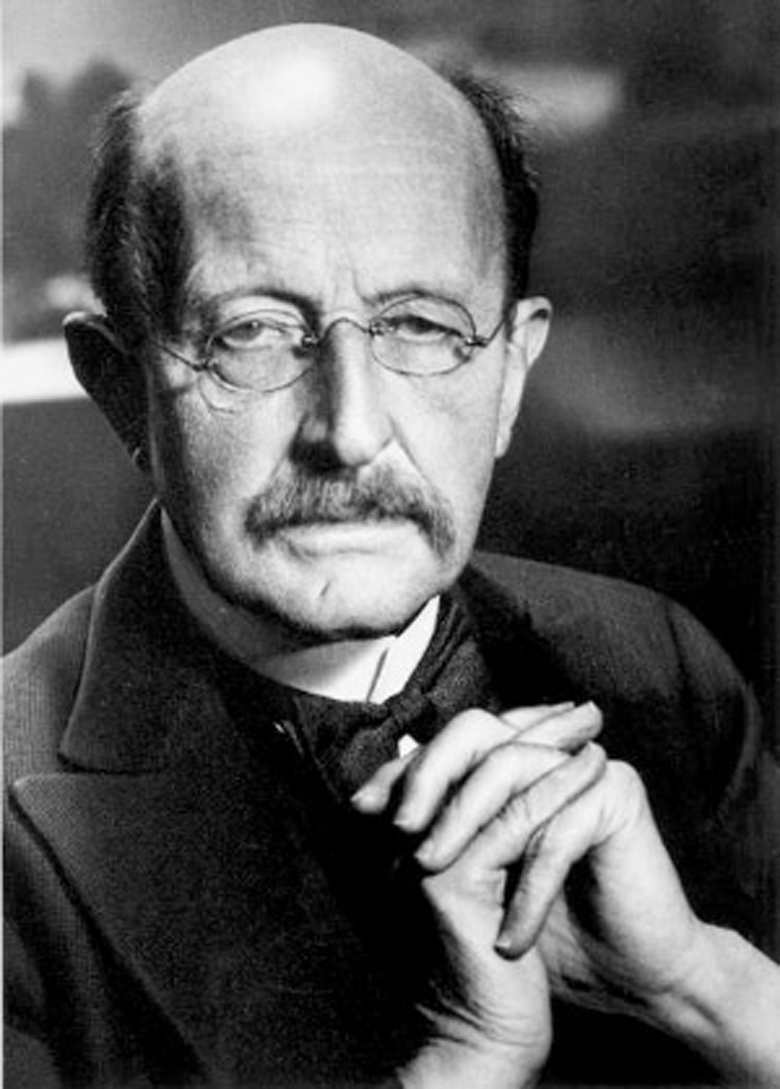
\includegraphics[width=\columnwidth]{img/planck.jpg}}
~
\visible<2->{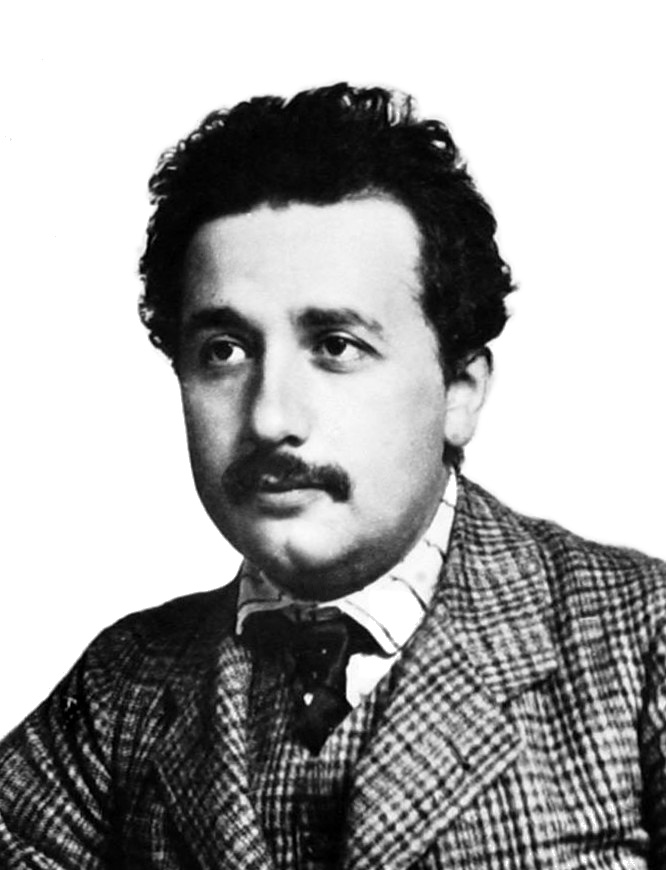
\includegraphics[width=\columnwidth]{img/einstein.jpg}}
\end{column}
\begin{column}{0.7\textwidth}
Nel XX secolo abbiamo ulteriori sviluppi:
\begin{itemize}
  \item<1-> Planck (1900) ipotizza che la radiazione elettromagnetica sia formata da \alert<1>{quanti di energia};
  \item<2-> Einstein (1905), analizzando l'effetto fotoelettrico, tratta la luce come flusso di particelle: i \alert<2>{fotoni}.
\end{itemize}
\end{column}
\end{columns}
\end{frame}


\begin{frame}
\frametitle{Dualismo onda-particella della luce}
\begin{figure}
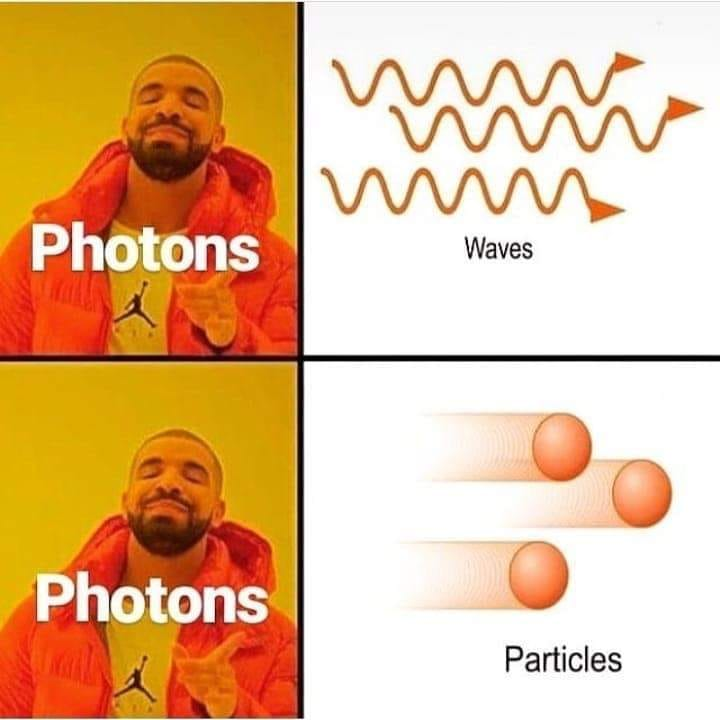
\includegraphics[width=.35\columnwidth]{img/photons.jpg}
\end{figure}
\begin{block}{Dualismo onda-particella della luce}
La luce si presenta come onda o come particella a seconda delle condizioni sperimentali.
\end{block}

\end{frame}

\section{De Broglie}

\begin{frame}
\frametitle{Un passo ulteriore}
\begin{columns}
\begin{column}{0.2\textwidth}
\visible<1->{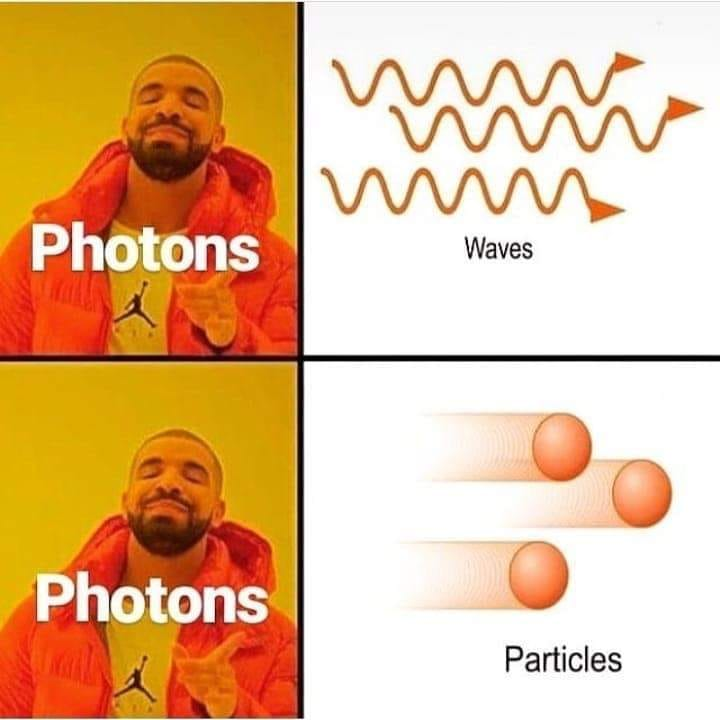
\includegraphics[width=\columnwidth]{img/photons.jpg}}
~
\visible<2->{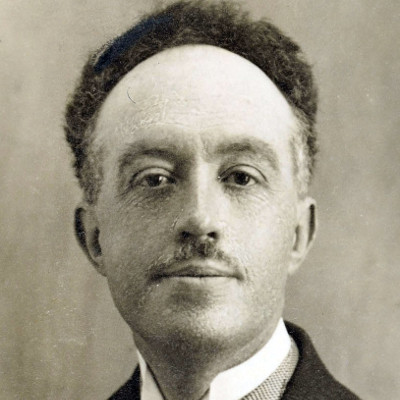
\includegraphics[width=\columnwidth]{img/debroglie.jpg}}
\end{column}
\begin{column}{0.7\textwidth}
~

~

~

A questo punto è lecito \alert<1>{chiedersi se vale lo stesso dualismo anche per la materia}, che abbiamo sempre pensato composta di particelle.\pause

~

~

Louis de Broglie (1924) scopre che \alert<2>{ad ogni particella con quantità di moto $ \vec{p} $ si associa una lunghezza d'onda $ \lambda $}:
\begin{center}
\colorbox{blue!30}{$ \lambda = \dfrac{h}{p} $}
\end{center}


\end{column}
\end{columns}
\end{frame}



\begin{frame}
\frametitle{Perché non ce ne siamo mai accorti?}
Per oggetti macroscopici, la \alert{lunghezza d'onda di de Broglie} è praticamente nulla.\pause

~

Per una cellula umana ($ m = 10^{-12} \, kg $) in moto a $ 1 \, \frac{cm}{s} = 10^{-2} \, \frac{m}{s} $:
\begin{center}
$ \lambda = \dfrac{h}{p} = \dfrac{h}{mv} = \dfrac{6,63 \times 10^{-34} \, Js}{10^{-12} \, kg \cdot 10^{-2} \, \frac{m}{s}} = 6,63 \times 10^{-20} \, m $
\end{center}\pause

~

Nel 2013 si è riusciti a dimostrare la proprietà di interferenza (e quindi la natura ondulatoria) di molecole con massa superiore a $ 10^4 \, uma = 1,66 \times 10^{-23} \, kg $.

\end{frame}


\begin{frame}
\frametitle{Analisi della relazione di de Broglie (1)}
Ricordiamo che, secondo Einstein, i fotoni hanno massa nulla e quantità di moto pari a $ p = \frac{E}{c} $.\pause

~

Sostituendo in $ \lambda = \dfrac{h}{p} $ otteniamo:
\begin{center}
$ \lambda = h \dfrac{c}{E} ~~~~~~\Longrightarrow~~~~~~ E = h \dfrac{c}{\lambda} $
\end{center}\pause
Ricordando che $ c = \lambda f $ e pertanto $ f = \dfrac{c}{\lambda} $:
\begin{center}
\colorbox{blue!30}{$ E = hf $}
\end{center}\pause
\alert{La relazione di Planck per i fotoni è pertanto conseguenza della relazione di de Broglie.}
\end{frame}





\begin{frame}
\frametitle{Esercizio}
\begin{exampleblock}{Collegare le formule tra loro}
\small{
  La lunghezza d'onda di de Broglie associata a un protone vale $ 7,0 \times 10^{-12} \, m $.
  
  Calcola il valore della differenza di potenziale che ha accelerato il protone.\hspace*{\fill}[$ 17 \, V $]
  }
\end{exampleblock}
\end{frame}





\begin{frame}
\frametitle{Analisi della relazione di de Broglie (2)}
La relazione di de Broglie permette anche di \alert<1>{giustificare l'ipotesi di quantizzazione delle orbite di Bohr}.\pause

~

Introduciamo un nuovo modello per l'elettrone, il \alert<2->{modello ondulatorio}.\pause

~

~

Un'onda stazionaria è un'onda che ha i nodi sempre nella stessa posizione dello spazio.
\begin{center}
\href{gif/ondastaz.gif}{\beamergotobutton{GIF: Onda stazionaria}}
\end{center}
\end{frame}

\begin{frame}
\frametitle{Modelli per l'elettrone}
\begin{columns}
\begin{column}{.4\textwidth}
\visible<1->{\begin{figure}
Modello corpuscolare

~

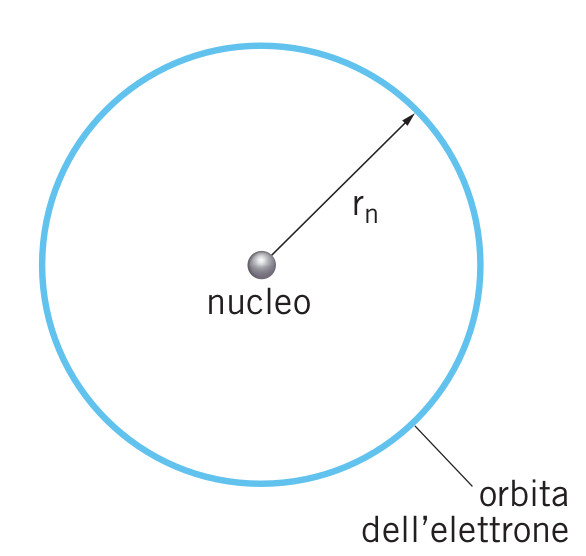
\includegraphics[width=.7\columnwidth]{img/modellocorp.jpg}
\end{figure}
L'elettrone si muove su un'orbita circolare di raggio $ r_n $ senza irraggiare.

~}
\end{column}
\begin{column}{.4\textwidth}
\visible<2>{\begin{figure}
Modello ondulatorio

~

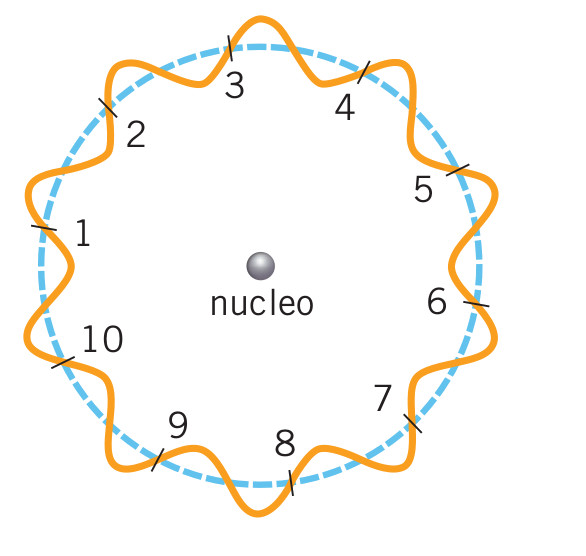
\includegraphics[width=.7\columnwidth]{img/modelloond.jpg}
\end{figure}
L'elettrone è un'onda stazionaria che deve ``chiudersi perfettamente su sé stessa''.}
\end{column}
\end{columns}
\end{frame}


\begin{frame}
\frametitle{Lunghezza d'onda di de Broglie nel modello ondulatorio}
\begin{figure}
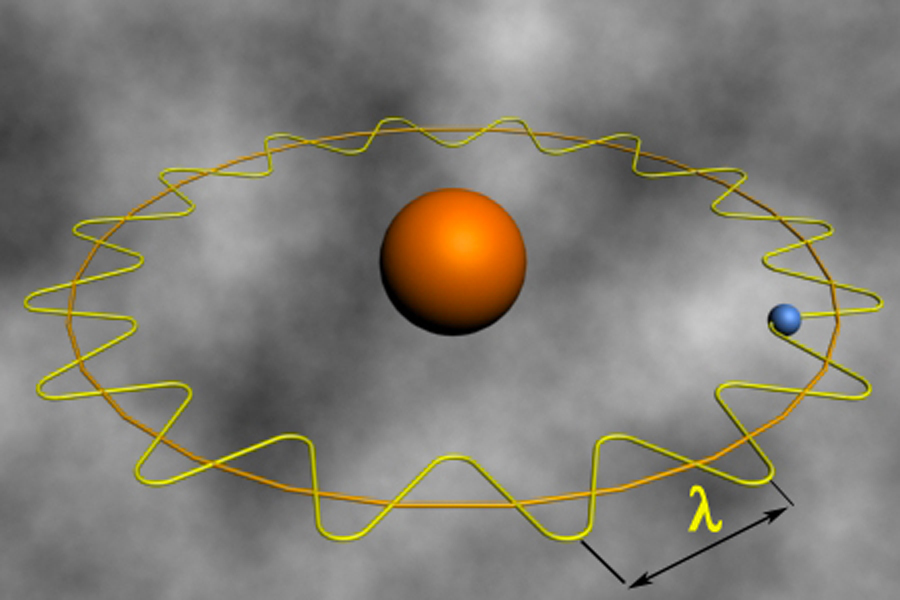
\includegraphics[width=.8\columnwidth]{img/elettronestaz.jpg}
\end{figure}
\end{frame}



\begin{frame}
\frametitle{Raggio dell'orbita e lunghezza d'onda di de Broglie}
Affinché l'onda risulti stazionaria, \alert<1>{la lunghezza dell'orbita deve essere un multiplo intero di $ \lambda $}:
\begin{center}
$ 2 \pi r_n = n \lambda $
\end{center}\pause
Con la relazione di de Broglie otteniamo:
\begin{center}
$ 2 \pi r_n = n \dfrac{h}{p} ~~~~~~ \Longrightarrow ~~~~~~ $\colorbox{blue!30}{$ 2 \pi r_n p = nh $}
\end{center}\pause
\alert{La relazione trovata è esattamente la condizione di quantizzazione di Bohr.}
\end{frame}

\section{Dualismo (2)}

\begin{frame}
\frametitle{Dualismo onda-particella}
\begin{block}{Dualismo onda-particella per luce e materia}
Sia la radiazione elettromagnetica, sia le particelle subatomiche mostrano in alcuni fenomeni natura ondulatoria, in altri natura corpuscolare.
\end{block}\pause

~

Ma abbiamo qualche conferma sperimentale del dualismo onda-particella per gli elettroni?
\end{frame}


\begin{frame}
\frametitle{L'esperimento di Davisson e Germer}
Nel 1927, Clinton Davisson e Lester Germer spararono elettroni contro un bersaglio di nichel cristallino.
\begin{figure}
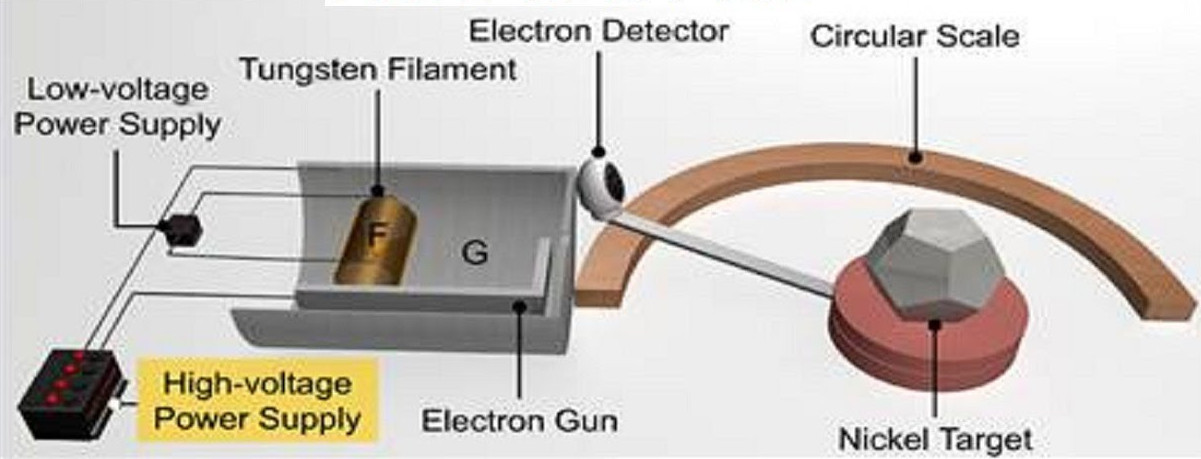
\includegraphics[width=.8\columnwidth]{img/davissongermer.jpg}
\end{figure}\pause
La velocità degli elettroni era tale che la lunghezza d'onda di de Broglie per gli elettroni risultava dello stesso odg della distanza tra gli atomi del cristallo.


\end{frame}

\begin{frame}
\frametitle{Risultati}

\alert{Gli elettroni venivano diffusi dal reticolo cristallino, formando una figura di diffrazione} (grazie al fenomeno dell'interferenza costruttiva e distruttiva, tipica delle onde).\pause

\visible<2>{
\begin{columns}
\begin{column}{.4\textwidth}
\begin{figure}
Diffusione degli elettroni

~

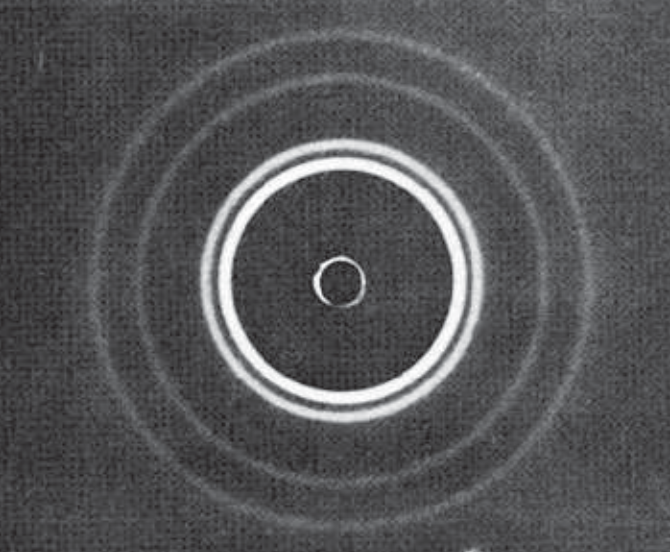
\includegraphics[width=\columnwidth]{img/diffelettroni.png}
\end{figure}
\end{column}
\begin{column}{.4\textwidth}
\begin{figure}
Diffusione dei raggi X

~

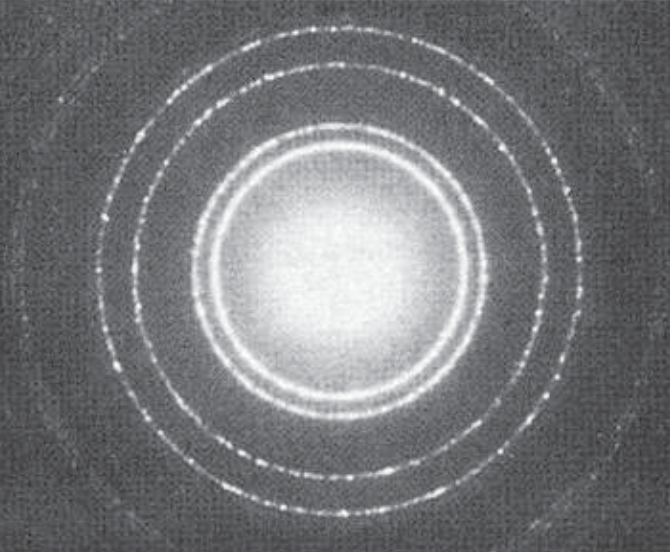
\includegraphics[width=\columnwidth]{img/diffraggix.png}
\end{figure}
\end{column}
\end{columns}}

\end{frame}


\begin{frame}
\frametitle{Confronto tra teoria ondulatoria e teoria corpuscolare}
\scriptsize
Se $ d $ è la dimensione degli oggetti con cui l'onda o le particelle interagiscono:

~

\centering
\begin{tabular}{p{5cm}|p{5cm}}
\textbf{Modello ondulatorio} & \textbf{Modello corpuscolare}\\\hline\rule{0pt}{3ex}
\hspace*{-.8em} l’onda è una perturbazione che trasporta energia in quantità discrete e se ne analizza la distribuzione di intensità & la particella è un corpuscolo a cui è associata la lunghezza d’onda di de Broglie e se ne analizzano gli scambi di energia e di quantità di moto \\\hline\rule{0pt}{3ex}
\hspace*{-.8em} $ \lambda < d $: la perturbazione si comporta come un insieme di pacchetti discreti di energia che può evidenziare 
l’aspetto corpuscolare (la luce nell’effetto fotoelettrico)  & $ \lambda < d $: la particella si comporta come un corpuscolo (gli elettroni nell’esperimento di Thomson)\\\hline\rule{0pt}{3ex}
\hspace*{-.8em} $ \lambda > d $: la perturbazione si comporta come un’onda con i tipici fenomeni di interferenza e diffrazione (la luce nell’esperimento di Young) & $ \lambda > d $: la particella presenta fenomeni ondulatori quali interferenza e diffrazione (gli elettroni nell’esperimento di Davisson e Germer) \\
\end{tabular}

\end{frame}



\section{Heisenberg}

\begin{frame}
\frametitle{Traiettoria}
In meccanica classica ogni particella segue una \alert<1-2>{traiettoria definita}, un tragitto lungo il quale possiamo specificare:
\begin{itemize}
  \item posizione;\pause
  \item velocità (e quindi quantità di moto).\pause
\end{itemize}

~

\alert<3>{Non si può determinare, invece, l’esatta localizzazione di una particella che si comporta come un’onda.}

~

L’elettrone dell’atomo di idrogeno non può essere descritto come una particella orbitante attorno al nucleo secondo una traiettoria definita.
\end{frame}



\begin{frame}
\frametitle{Una confusione da evitare}

\begin{figure}
\begin{tikzpicture}[scale=.6,samples=100]
\draw[smooth, blue, ultra thick, domain=0:1.5*pi] plot (\x, {.6*sin(4* \x r)});
\draw[purple, ultra thick,fill=purple] (-3,0) circle [radius=.2];
\node[below,purple] at (-3,-1) {particella};
\node[below,blue] at (2.36,-1) {onda};
\end{tikzpicture}
\end{figure}
\begin{quote}\begin{small}
Esaminando i due disegni, un profano potrebbe forse pensare che che il disegno a destra rappresenta semplicemente una particella che si muove seguendo una forma d'onda. Tuttavia, questa considerazione nasce dall'aver frainteso il concetto di onda. [\ldots] Ciò che viene trasportato dall'onda è la perturbazione che provoca il fenomeno ondulatorio, ma non particelle materiali. Nella meccanica quantistica, perciò, non ci riferiamo alla traiettoria di una particella quando diciamo che la particella è anche un'onda. Ciò che intendiamo è che la forma d'onda nel suo insieme è una manifestazione della particella.

\begin{flushright}
F.~Capra, \emph{Il Tao della fisica}
\end{flushright}
\end{small}\end{quote}

\end{frame}


\begin{frame}
\frametitle{Il principio di indeterminazione (1)}
Werner Heisenberg elabora nel 1925 (insieme a Max Born e Pascual Jordan) una \alert<1>{meccanica delle matrici}, la prima formulazione logicamente coerente e autonoma della meccanica quantistica.\pause

~

Dalla sua meccanica, Heisenberg dimostra l'impossibilità di misurare con precisione la posizione di un elettrone \alert{e} la sua quantità di moto.
\end{frame}

\begin{frame}
\frametitle{Il principio di indeterminazione (2)}
\begin{block}{Principio di indeterminazione}
È impossibile definire ad un certo istante la posizione di una particella e la sua quantità di moto.
\begin{center}
\colorbox{blue!30}{$ \Delta x \Delta p \simeq \dfrac{\hbar}{2} $}
\end{center}
$ \Delta x = $ incertezza sulla posizione

$ \Delta p = $ incertezza sulla quantità di moto

$ \hbar = \frac{h}{2\pi} $ = costante di Planck ridotta (acca tagliato)
\end{block}\pause
\alert<2>{$ \Delta x $ e $ \Delta p $ sono inversamente proporzionali.}

~

Possiamo conoscere con precisione la posizione di una particella, ma non la sua velocità (e viceversa).
\end{frame}

\begin{frame}
\frametitle{Interpretare Heisenberg}
Nella fisica classica, una misura è soggetta ad una indeterminazione dovuta alle \alert<1>{caratteristiche degli strumenti}.\pause

~

Con il miglioramento degli strumenti, l’imprecisione diminuisce e l’unico ostacolo è costituito dalle \alert<2>{capacità tecnologiche}.\pause

~

Il principio di indeterminazione non è dovuto ad effetti di disturbo dovuti all'esecuzione delle misure, e non rappresenta un'incertezza sperimentale rispetto a un valore ``vero''.

~

\alert{L'indeterminazione è una proprietà intrinseca dei sistemi quantistici.}
\end{frame}


\begin{frame}
\frametitle{Perché non ce ne siamo mai accorti?}
Per gli oggetti macroscopici, la indeterminazioni $ \Delta x $ e $ \Delta p $ sono trascurabili rispetto agli errori di misura.
\end{frame}



\begin{frame}
\frametitle{Formulazione alternativa}
\begin{block}{Principio di indeterminazione (seconda formulazione)}
La precisione con cui si misura l'energia di una particella è inversamente proporzionale al tempo della misurazione.
\begin{center}
\colorbox{blue!30}{$ \Delta E \Delta t \simeq \dfrac{\hbar}{2} $}
\end{center}
$ \Delta E, \Delta t = $ incertezza sull'energia, incertezza sul tempo
\end{block}
\end{frame}


\section{Schr\"odinger}

\begin{frame}
\frametitle{La funzione d'onda (1)}
Chiamiamo $ \Psi (x,y,z,t) $ la funzione che rappresenta un'onda di de Broglie.\pause

~

Sappiamo che lo stato di un sistema può essere descritto mediante la sua energia:
\[ E_{tot} = K+U \]\pause
Erwin Schr\"odinger nel 1926 riuscirà a ottenere l'analogo quantistico di tale relazione:
\[ i \hbar \frac{\partial \Psi(x,t)}{\partial t} = - \frac{\hbar^2}{2m} \frac{\partial^2 (x,t)}{\partial x^2} + V(x,t)\Psi(x,t)   \]
\end{frame}


\begin{frame}
\frametitle{La funzione d'onda (2)}
\[ i \hbar \frac{\partial \Psi(x,t)}{\partial t} = - \frac{\hbar^2}{2m} \frac{\partial^2 (x,t)}{\partial x^2} + V(x,t)\Psi(x,t)   \]

~

Le soluzioni dell'equazione (differenziale) di Schr\"odinger sono le funzioni d'onda che permettono di descrivere le proprietà quantistiche del sistema.

~

Secondo Schr\"odinger, un elettrone (ad esempio) non si comporta come un punto materiale, ma ha una "esistenza distribuita" in un certo volume di spazio.
\end{frame}


\begin{frame}
\frametitle{Interpretazione di Born}
Max Born propose un'\alert<1>{interpretazione probabilistica} delle funzioni d'onda.\pause

~

Fissato un istante di tempo $ t $, la probabilità che un elettrone occupi un certo volume di spazio $ \Delta V $ è data da:
\[P(t) = |\Psi (x,y,z,t)|^2\Delta V \]
\end{frame}

\begin{frame}
\frametitle{Pacchetti d'onda}
La fisica quantistica abbandona pertanto il concetto di particella in favore di quello di \alert{pacchetto d'onda} (wave packet).
\begin{figure}
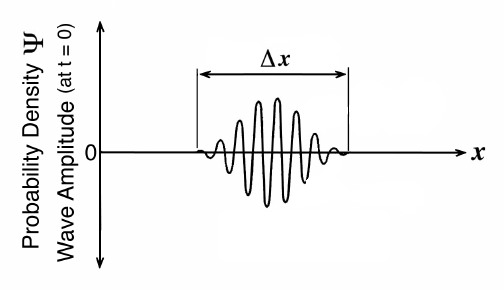
\includegraphics[width=.7\columnwidth]{img/pacchettoonda.png}
\end{figure}
\end{frame}


\begin{frame}
\frametitle{L'interpretazione di Copenhagen (1926-27)}
Proposta da Bohr e Heisenberg estendendo le idee di Born, si basa sul fatto che un sistema quantistico ha in generale più stati possibili, ciascuno descritto da una funzione d'onda. Ogni stato è detto \alert{stato quantico}.\pause

~

Gli stati quantici sono ``sovrapposti'' gli uni agli altri.\pause

~

\begin{columns}
\begin{column}{0.2\textwidth}
\visible<3->{\begin{figure}

\includegraphics[width=\columnwidth]{img/gattoschrodinger.jpeg}
\end{figure}}
\end{column}
\begin{column}{0.7\textwidth}
L'atto della misurazione fa collassare lo stato di sovrapposizione in uno degli stati fondamentali.\pause

~

È quindi la misurazione stessa che ``estrae'' uno tra i valori possibili di $ \Psi $.
\end{column}
\end{columns}

\end{frame}

\end{document}
